% Why Should This Work? -- slides around the notebook: slides, then the notebook, then slides.
% Figures and every number quoted here come from why_should_this_work_figures.py,
% which uses the same data and calculations as chapters/Finance/L9_WhyShouldThisWork_AI.ipynb.
\documentclass[aspectratio=169,10pt]{beamer}
\usetheme{default}
\usecolortheme{default}

\usepackage{graphicx}
\usepackage{adjustbox}
\usepackage{amsmath}
\usepackage{amssymb}
\usepackage{booktabs}
\usepackage{array}
\newcolumntype{P}[1]{>{\raggedright\arraybackslash}p{#1}}
\usepackage{tikz}
\usetikzlibrary{arrows.meta,positioning,calc,shadows}
\usepackage{appendixnumberbeamer}  % Exclude appendix from slide count

\setbeamertemplate{navigation symbols}{}
\setbeamertemplate{items}[circle]

% Footline: Author, Event (Year) on left; page/total on right
\setbeamertemplate{footline}{
  \hbox{%
    \begin{beamercolorbox}[wd=.5\paperwidth,ht=2.5ex,dp=1ex,left]{author in head/foot}%
      \hspace*{2ex}\insertshortauthor, \insertshortinstitute\ (\insertdate)
    \end{beamercolorbox}%
    \begin{beamercolorbox}[wd=.5\paperwidth,ht=2.5ex,dp=1ex,right]{date in head/foot}%
      \insertframenumber/\inserttotalframenumber\hspace*{2ex}
    \end{beamercolorbox}%
  }
}

% Highlight boxes
\setbeamercolor{box1}{bg=red!12,fg=black}

% A poll option: {colour}{letter and choice}  (same as the Hiring and Firing deck)
\newcommand{\pollbox}[2]{\tikz\node[draw=#1!65!black, fill=#1!10, rounded corners=4pt, minimum width=3.7cm,
                                   minimum height=1.1cm, align=center, font=\large]{#2};}
\newcommand{\bignum}[1]{{\fontsize{44}{48}\selectfont\textbf{\textcolor{red!75!black}{#1}}}}

\title{Why Should This Work?}
\subtitle{Once the backtest is honest, what is left is economics}
\author[A. Moreira]{Alan Moreira}
\institute[Data-Driven Investing]{NYU Stern --- Data-Driven Investing}
\date{Fall 2026}

\begin{document}

%================================================================== PART 1: SLIDES
%------------------------------------------------------------------ 1
\begin{frame}
\titlepage
\end{frame}

%------------------------------------------------------------------ 2
\begin{frame}{Monday: the record you are shown was selected}
\begin{itemize}
\item The managers who come to see you are the ones whose record cleared the bar
\vskip 12pt
\item Journals work the same way: they print the strategies whose t-statistic cleared the bar
\end{itemize}
\vskip 20pt
\begin{beamercolorbox}[rounded=true,sep=8pt,center]{box1}
Today: the published record, and what is left to ask once the backtest is honest
\end{beamercolorbox}
\end{frame}

%------------------------------------------------------------------ 3
\begin{frame}{Today's question}
\vskip 10pt
\begin{center}
{\Large Why should anyone pay you a premium for holding this?}
\end{center}
\vskip 24pt
\begin{itemize}
\item Statistics can tell you a strategy made money. It cannot tell you why it should keep making it.
\vskip 10pt
\item That takes a story: \textbf{who is on the other side of the trade, and why they are willing}
\end{itemize}
\end{frame}

%------------------------------------------------------------------ 4
\begin{frame}{Predict first: how many survive?}
27 of our strategies were published with a significant t-statistic. Re-run on our sample, 1980--2000:
\vskip 6pt
\begin{center}
{\large How many clear the Bonferroni bar, $|t| > 3.11$?}
\end{center}
\vskip 10pt
\begin{center}
\pollbox{blue}{\textbf{A}\ \ 0 to 6} \hspace{6pt}
\pollbox{blue}{\textbf{B}\ \ 7 to 13} \\[8pt]
\pollbox{blue}{\textbf{C}\ \ 14 to 20} \hspace{6pt}
\pollbox{blue}{\textbf{D}\ \ 21 to 27}
\end{center}
\vskip 6pt
Write your answer down. You will type it into the notebook, and the notebook will tell you.
\end{frame}

%------------------------------------------------------------------ 5
\begin{frame}{Predict first: three papers, how many trades?}
Three volatility papers, two sets of authors: idiosyncratic volatility and realized volatility (Ang et al.\ 2006), and lottery-like stocks (Bali, Cakici and Whitelaw 2011).
\vskip 6pt
\begin{center}
{\large How correlated are their long-short returns?}
\end{center}
\vskip 10pt
\begin{center}
\pollbox{gray}{\textbf{A}\ \ below 0.3} \hspace{6pt}
\pollbox{gray}{\textbf{B}\ \ 0.3 to 0.6} \\[8pt]
\pollbox{gray}{\textbf{C}\ \ 0.6 to 0.9} \hspace{6pt}
\pollbox{gray}{\textbf{D}\ \ above 0.9}
\end{center}
\end{frame}

%================================================================== PART 2: THE NOTEBOOK
%------------------------------------------------------------------ 6
\begin{frame}{Now: the notebook}
\vskip 2pt
\begin{beamercolorbox}[rounded=true,sep=7pt,center]{box1}
\textbf{Notebook: Why Should This Work? (in class)} \ --- \ about 30 minutes, in pairs
\end{beamercolorbox}
\vskip 10pt
\begin{enumerate}
\item \textbf{§1 The gap.} Type your first prediction, then run the replication table.
\vskip 5pt
\item \textbf{§2 Count ideas, not papers.} Type your second prediction, then run the volatility family.
\vskip 5pt
\item \textbf{§3 Prompt it.} \emph{``What was the worst drawdown?''} Write the prompt, then run the check and read the code.
\vskip 5pt
\item \textbf{§4 Your strategy.} Its closest neighbours, and its worst episode: one line to write.
\end{enumerate}
\vskip 8pt
{\small \textbf{Note:} cells marked with a lock run as they are. Stop at \textbf{Back to the slides}; everything after it (§5 onwards) is for after class.}
\end{frame}

%================================================================== PART 3: SLIDES
%------------------------------------------------------------------ 7
\begin{frame}{Six of 27 survive}
\begin{center}
\adjustbox{max width=0.85\textwidth, max height=0.6\textheight}{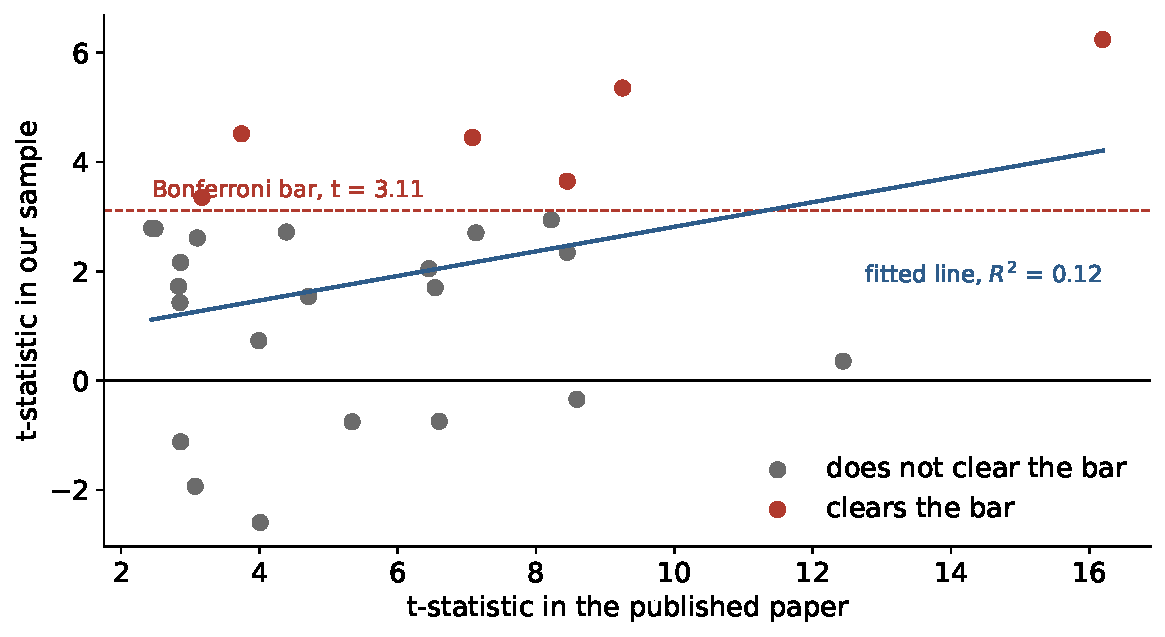
\includegraphics{figures/wstw_replication.pdf}}
\end{center}
\vskip -2pt
\begin{itemize}
\item Six come out with the \textbf{wrong sign}. The published t explains \textcolor{red}{12\%} of ours.
\vskip 3pt
\item Knowing a paper reported $t = 9$ rather than $t = 3$ tells you almost nothing about what you will get
\end{itemize}
\end{frame}

%------------------------------------------------------------------ 8
\begin{frame}{Three explanations, one table}
\begin{center}
\renewcommand{\arraystretch}{1.6}
\begin{tabular}{l P{6.6cm} l}
\toprule
 & mechanism & so the effect \dots \\
\midrule
\textbf{Selection} & journals print what worked; the failures stay in a drawer & never existed \\
\textbf{Overfitting} & the authors searched too & never existed \\
\textbf{Decay} & it was real; publication revealed it; investors traded it away & existed, and is gone \\
\bottomrule
\end{tabular}
\end{center}
\vskip 12pt
\begin{beamercolorbox}[rounded=true,sep=8pt,center]{box1}
A replication gap cannot tell you which. Two say never trade it; one says you are late.
\end{beamercolorbox}
\end{frame}

%------------------------------------------------------------------ 9
\begin{frame}{Risk for whom?}
\begin{itemize}
\item Risk is not a property of an asset. It is a property of an asset \textbf{for a particular investor}.
\vskip 12pt
\item You are paid to hold something that \textbf{pays off badly in bad times}, when you can least afford it
\vskip 12pt
\item The CAPM is one narrow version: it declares that bad times means the market falling
\vskip 12pt
\item But bad times are about people: a lost job, a house that falls with the market, a credit line that disappears
\end{itemize}
\end{frame}

%------------------------------------------------------------------ 10
\begin{frame}{Differ from the market only if you differ}
You work in the auto industry. Your income already moves with autos, so hold \textbf{the market minus autos}.
\vskip 8pt
\begin{center}
\renewcommand{\arraystretch}{1.6}
\begin{tabular}{P{4.7cm} P{4.1cm} P{3.9cm}}
\toprule
 & & what you should do \\
\midrule
\textbf{You are the average investor} & your bad times are the market's & hold the market \\
\textbf{You genuinely differ} & what scares them does not scare you & take the other side, and get paid \\
\textbf{You think you differ, and do not} & the most common case & you find out at the worst time \\
\bottomrule
\end{tabular}
\end{center}
\vskip 6pt
\begin{itemize}
\item Two investors can agree on every statistic and still correctly reach opposite decisions
\end{itemize}
\end{frame}

%------------------------------------------------------------------ 11
\begin{frame}{As you scale, you become the investor bearing the risk}
\begin{itemize}
\item ``Risky for them, not for me'' is a statement about a \textbf{small} position
\vskip 12pt
\item Put enough capital behind it, and you are the one holding through the drawdown and meeting the margin call
\vskip 12pt
\item If everyone held it, prices would adjust and the premium would shrink
\end{itemize}
\vskip 16pt
\begin{beamercolorbox}[rounded=true,sep=8pt,center]{box1}
Can the world support everyone picking up this \$100 bill?
\end{beamercolorbox}
\end{frame}

%------------------------------------------------------------------ 12
\begin{frame}{A high expected return is a low price}
``These stocks earn more'' is the same sentence as \textbf{``these stocks are cheap''}. Someone is selling to you at that price.
\vskip 8pt
\begin{center}
\renewcommand{\arraystretch}{1.6}
\begin{tabular}{l P{5.6cm} P{4.6cm}}
\toprule
 & why the price is low & what you are buying \\
\midrule
\textbf{Cash flows} & the market expects the business to do badly, and is right & a bad business at a fair price \\
\textbf{Risk} & it pays off badly when investors care most & compensation for bearing something real \\
\bottomrule
\end{tabular}
\end{center}
\vskip 8pt
\begin{beamercolorbox}[rounded=true,sep=7pt,center]{box1}
Who is selling to you, and what makes them willing? If you cannot name them, you are the one being selected.
\end{beamercolorbox}
\end{frame}

%------------------------------------------------------------------ 13
\begin{frame}{Low volatility: who is on the other side?}
\begin{itemize}
\item \textbf{The claim:} quiet, low-beta stocks earn more than their risk justifies
\vskip 10pt
\item \textbf{The counterparty:} investors who want equity-like returns but cannot borrow (mandates, regulation, margin). To reach for return, they buy risky stocks.
\vskip 10pt
\item That bids up the volatile names and leaves the quiet ones cheap
\vskip 10pt
\item Their reason is a \textcolor{red}{constraint}, not a mistake. Constraints do not go away because someone points them out.
\end{itemize}
\vskip 6pt
\begin{itemize}
\item Is it risky for \emph{you}? Only if you are unconstrained: if you can borrow, and if you can hold.
\end{itemize}
\end{frame}

%------------------------------------------------------------------ 14
\begin{frame}{What holding it felt like}
\begin{center}
\adjustbox{max width=0.85\textwidth, max height=0.6\textheight}{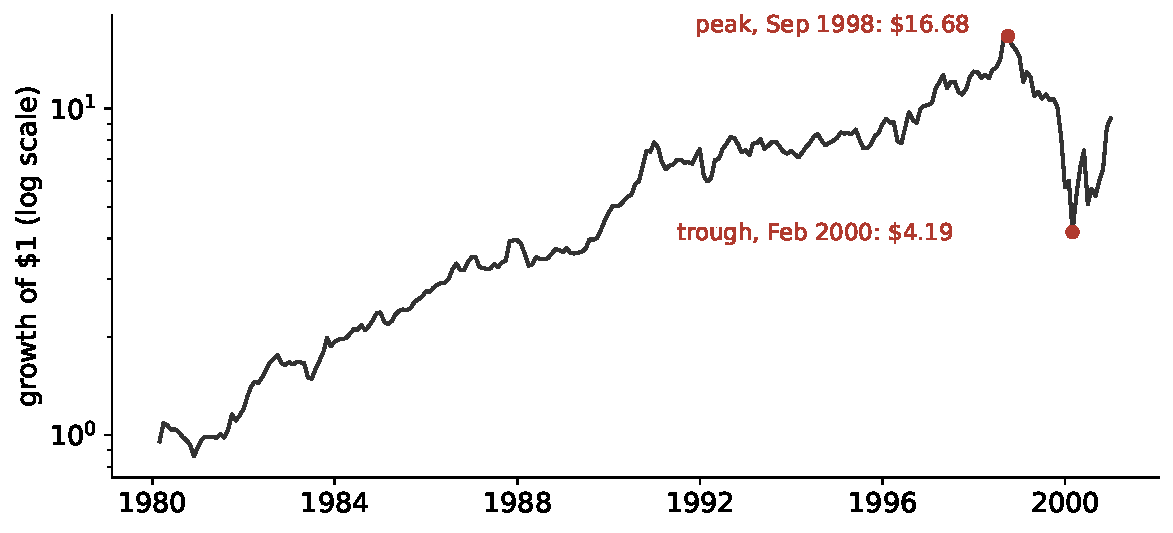
\includegraphics{figures/wstw_lowvol_growth.pdf}}
\end{center}
\vskip -2pt
\begin{itemize}
\item 15.4\% a year from 1980 to 1997. Then 1999: \textcolor{red}{$-60\%$}.
\vskip 3pt
\item The strategy is short lottery stocks, and in a bubble lottery stocks are exactly what runs
\end{itemize}
\end{frame}

%------------------------------------------------------------------ 15
\begin{frame}{Leverage turned a bad year into a wipeout}
\begin{center}
\adjustbox{max width=0.85\textwidth, max height=0.6\textheight}{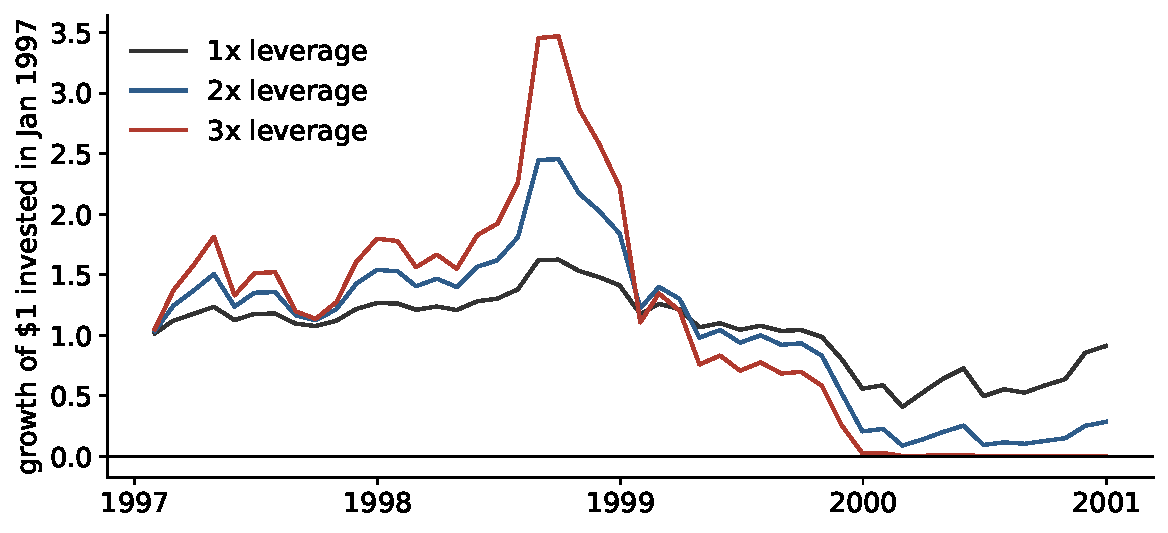
\includegraphics{figures/wstw_leverage.pdf}}
\end{center}
\vskip -2pt
\begin{itemize}
\item At 2$\times$ you lose 96\%. At 3$\times$ you are wiped out in \textcolor{red}{June 2000}, before the recovery.
\vskip 3pt
\item Harvesting this premium needed leverage. The risk that was other people's became yours when you scaled.
\end{itemize}
\end{frame}

%------------------------------------------------------------------ 16
\begin{frame}{Overfitting, or the premium being paid?}
\begin{itemize}
\item In the backtesting lecture this was the in-sample winner: Sharpe ratio \textbf{1.37} in 1980--1990, \textbf{0.22} in 1991--2000
\vskip 12pt
\item \textbf{If it is overfitting:} drop it
\vskip 8pt
\item \textbf{If it is the premium being paid for:} the bad state the story predicts arrived. Size it to survive the next 1999.
\end{itemize}
\vskip 16pt
\begin{beamercolorbox}[rounded=true,sep=8pt,center]{box1}
Nothing in the returns tells you which. Only a story written down beforehand does.
\end{beamercolorbox}
\end{frame}

%------------------------------------------------------------------ 17
\begin{frame}{Worked problem: what was the worst drawdown?}
A long-short strategy earns these returns over four months:
\vskip 6pt
\begin{center}
\renewcommand{\arraystretch}{1.4}
\begin{tabular}{ccccc}
\toprule
month & 1 & 2 & 3 & 4 \\
\midrule
return & $+10\%$ & $-20\%$ & $-20\%$ & $+5\%$ \\
\bottomrule
\end{tabular}
\end{center}
\vskip 10pt
\begin{enumerate}
\item[(a)] Worst drawdown, funded 1-for-1 with equity, compounded
\vskip 6pt
\item[(b)] The same at 2$\times$ leverage
\vskip 6pt
\item[(c)] The same, summing the returns instead of compounding
\end{enumerate}
\vskip 10pt
{\small Work it by hand. The notebook's §5 has a cell to check it.}
\end{frame}

%------------------------------------------------------------------ 18
\begin{frame}{Worked problem: three answers from the same returns}
\begin{center}
\renewcommand{\arraystretch}{1.4}
\begin{tabular}{lccccc}
\toprule
value after month & 1 & 2 & 3 & 4 & worst drawdown \\
\midrule
(a) 1$\times$, compounded & 1.10 & 0.88 & 0.704 & 0.739 & $0.704 / 1.10 - 1 = $ \textcolor{red}{$-36\%$} \\
(b) 2$\times$, compounded & 1.20 & 0.72 & 0.432 & 0.475 & $0.432 / 1.20 - 1 = $ \textcolor{red}{$-64\%$} \\
(c) summing returns & $+10$ & $-10$ & $-30$ & $-25$ & $-30 - 10 = -40$ points \\
\bottomrule
\end{tabular}
\end{center}
\vskip 12pt
\begin{itemize}
\item A long-short has no capital of its own. A drawdown is undefined until you say what capital you posted.
\vskip 6pt
\item Leverage deepens the same loss: $-36\%$ at 1$\times$, $-64\%$ at 2$\times$, $-84\%$ at 3$\times$
\end{itemize}
\end{frame}

%------------------------------------------------------------------ 19
\begin{frame}{Five questions before you trade a signal}
\begin{enumerate}
\item \textbf{Who is on the other side}, and what makes them willing?
\vskip 8pt
\item Is their reason a \textbf{constraint, a preference, or an error}? Constraints persist; errors get arbitraged.
\vskip 8pt
\item Is the risk one \textbf{you} can bear, at the size you intend to trade?
\vskip 8pt
\item What would you have to see to stop believing? \textbf{Name it now}, while it is cheap.
\vskip 8pt
\item If the answer to (1) is ``I don't know'', \textbf{you are the counterparty}
\end{enumerate}
\end{frame}

%------------------------------------------------------------------ 20
\begin{frame}{Homework: the valuation family}
Do to value what we did to volatility: book-to-market (\texttt{BM}), earnings-to-price (\texttt{EP}) and the enterprise multiple (\texttt{EntMult}). Three papers, three decades.
\vskip 8pt
\begin{enumerate}
\item[Q1] \textbf{How many ideas is this?} The mean pairwise correlation of the three
\vskip 4pt
\item[Q2] \textbf{The worst episode.} The composite's drawdown, funded 1-for-1, compounded, and when it happened
\vskip 4pt
\item[Q3] \textbf{Is it a hedge?} The composite's market beta
\vskip 4pt
\item[Q4] \textbf{The memo.} How many bets is this, and who is on the other side of the value trade: a constraint, a preference, or an error?
\end{enumerate}
\vskip 6pt
{\small Same steps as today's volatility family. It is at the end of today's notebook, after §5. Due before the next class.}
\end{frame}

%------------------------------------------------------------------ 21
\begin{frame}{Takeaways}
\begin{itemize}
\item A replication gap has three explanations, and the data cannot separate them
\vskip 7pt
\item Count ideas, not papers: three volatility papers are one trade
\vskip 7pt
\item Risk is a property of an asset \textbf{for an investor}. Deviate from the market only if you differ.
\vskip 7pt
\item A high expected return is a low price: ask who is selling, and why
\vskip 7pt
\item As you scale, you become the investor bearing the risk
\vskip 7pt
\item A drawdown is undefined for a long-short until you say what capital you posted
\end{itemize}
\end{frame}

\end{document}
